% ============================================================================
%  Neural World Models for a Grid Game: Santa's Gift Journey
%  Beamer deck — compiles on Overleaf (pdfLaTeX). No external image files needed.
%  Drop your own frames into \graphicspath and uncomment the \includegraphics
%  lines marked  % <-- FIGURE  to add screenshots.
% ============================================================================
\documentclass[aspectratio=169,11pt]{beamer}

\usetheme{metropolis}                 % clean, modern, IIT-seminar friendly
\usecolortheme{seahorse}
\metroset{progressbar=frametitle, sectionpage=progressbar, numbering=fraction}

\usepackage{booktabs}
\usepackage{tikz}
\usetikzlibrary{arrows.meta,positioning,shapes.geometric,fit,backgrounds}
\usepackage{xcolor}
\usepackage{amsmath}
\usepackage{fontawesome5}

% --- palette pulled from the game (Santa-badge red, winter slate, pine) -------
\definecolor{badge}{HTML}{C62828}
\definecolor{pine}{HTML}{2E7D5B}
\definecolor{amber}{HTML}{C0873A}
\definecolor{slate}{HTML}{3D6EA5}
\definecolor{ink}{HTML}{16212E}
\setbeamercolor{frametitle}{bg=ink,fg=white}
\setbeamercolor{progress bar}{fg=badge}
\setbeamercolor{alerted text}{fg=badge}

\newcommand{\hit}{\textcolor{pine}{\faCheckCircle}}
\newcommand{\miss}{\textcolor{amber}{\faTimesCircle}}
\newcommand{\code}[1]{\texttt{\small #1}}

\title{Learning to Play a Grid Game with a Diffusion World Model}
\subtitle{Spatial control, latency, and why a 6.8M model beat a 4B one}
\author{Spatial-Intel}
\date{\today}
\institute{Santa's Gift Journey \textbullet\ next-frame prediction from (frame, action)}

\begin{document}

\maketitle

% ---------------------------------------------------------------------------
\begin{frame}{The problem}
  \textbf{Task.} Given a game frame and a move action (up/down/left/right),
  predict the \emph{next} frame with the red ``S'' badge relocated one cell ---
  a learned \alert{world model}, not scripted pixel edits.

  \vspace{0.6em}
  \begin{columns}[T]
    \column{0.55\textwidth}
      Why it is hard:
      \begin{itemize}
        \item The moved object (badge) is \alert{$\sim$4\%} of a busy 1024px scene
              (houses, presents, trees, snow).
        \item Whole-image loss \emph{drowns} the move signal in background reconstruction.
        \item We want it \alert{fast} --- benchmarking latency at every stage.
      \end{itemize}
    \column{0.42\textwidth}
      \centering
      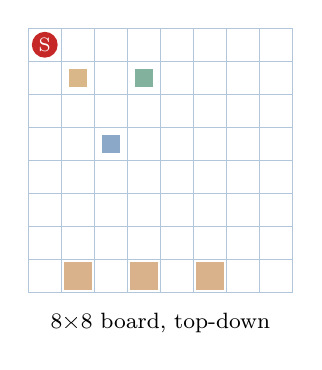
\begin{tikzpicture}[scale=0.42, every node/.style={font=\scriptsize}]
        \draw[step=1,slate!40,thin] (0,0) grid (8,8);
        \node[circle,fill=badge,text=white,inner sep=1pt] at (0.5,7.5) {S};
        \node[fill=amber!60,minimum size=6pt] at (1.5,6.5) {};
        \node[fill=pine!60,minimum size=6pt] at (3.5,6.5) {};
        \node[fill=slate!60,minimum size=6pt] at (2.5,4.5) {};
        \foreach \x in {1.5,3.5,5.5} \node[fill=brown!60,minimum size=10pt] at (\x,0.5) {};
        \node at (4,-0.9) {\footnotesize 8\texttimes8 board, top-down};
      \end{tikzpicture}
  \end{columns}
\end{frame}

% ---------------------------------------------------------------------------
\section{The data}
\begin{frame}{The data}
  \begin{columns}[T]
    \column{0.5\textwidth}
      \textbf{Source.} Deterministic game renderer (\code{SantaEnv}, $\sim$1\,ms,
      pixel-exact) --- Gemini image-editing was \alert{tested and rejected}:
      even on valid single-cell moves it misplaced the badge by several cells.
      \vspace{0.5em}
      \begin{itemize}
        \item \textbf{6 real moves} $\times$ 20 --- \code{data/santa\_real}
        \item \textbf{9-move playthrough} --- a coherent walk
              $(1,1)\!\to\!(4,1)\!\to\!(4,7)$, ending on house B
      \end{itemize}
    \column{0.5\textwidth}
      \centering\small
      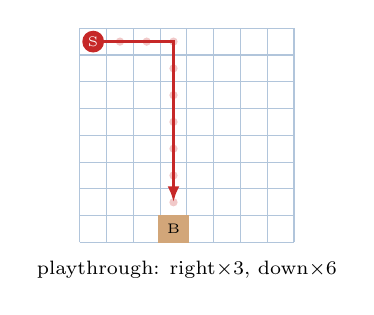
\begin{tikzpicture}[scale=0.34, every node/.style={font=\tiny}]
        \draw[step=1,slate!40] (0,0) grid (8,8);
        % walk: right x3 along top row, then down col 4
        \foreach \x/\y in {0/7,1/7,2/7,3/7,3/6,3/5,3/4,3/3,3/2,3/1}
          \node[circle,fill=badge!25,minimum size=3pt,inner sep=0pt] at (\x+0.5,\y+0.5) {};
        \draw[-{Latex[length=2mm]},badge,very thick]
          (0.5,7.5) -- (3.5,7.5) -- (3.5,1.5);
        \node[circle,fill=badge,text=white,inner sep=1pt] at (0.5,7.5) {S};
        \node[fill=brown!70,minimum size=9pt] at (3.5,0.5) {B};
        \node at (4,-1) {\scriptsize playthrough: right$\times$3, down$\times$6};
      \end{tikzpicture}
  \end{columns}
  \vspace{0.4em}
  \footnotesize\alert{Key insight:} the label source \emph{must} be exact ---
  a noisy teacher (Gemini) cannot teach precise spatial dynamics.
\end{frame}

% ---------------------------------------------------------------------------
\section{What we searched}
\begin{frame}{What we searched: RL \& verifiable rewards for diffusion}
  We surveyed how to fine-tune flow-matching / diffusion models for a
  \emph{verifiable} spatial objective:
  \vspace{0.4em}
  \begin{itemize}
    \item \textbf{DDPO / DPOK} --- RL fine-tuning of diffusion as a policy.
    \item \textbf{Flow-GRPO / DanceGRPO} --- GRPO adapted to flow-matching samplers.
    \item \textbf{RLVR} (verifiable rewards): \code{+1} correct placement, \code{-1} else.
    \item \textbf{RLVR-World} (arXiv:2505.13934), \textbf{VideoRLVR / SDE-GRPO} ---
          confirmed RLVR \emph{on diffusion world models} exists.
    \item \textbf{VLM-as-reward} --- InternVL / Qwen2.5-VL to emit JSON cell detection.
  \end{itemize}
  \vspace{0.3em}
  \footnotesize Finding: no off-the-shelf GRPO supports FLUX.2-klein; a verifiable
  reward needs a reliable cell detector first --- which itself became a theme.
\end{frame}

\begin{frame}{What we searched: why every edit model \emph{copied} the input}
  Literature on neural game engines explained the failure mode we kept hitting:
  \vspace{0.5em}
  \begin{block}{DIAMOND (NeurIPS 2024) + GameNGen (2024)}
    \begin{itemize}
      \item Action must enter as a \alert{FiLM embedding in every UNet block} ---
            \emph{not} a weak text prompt.
      \item Context frame \alert{channel-concatenated} --- not a copyable input image.
      \item \alert{High-noise-biased} $\sigma$ sampling ($P_{\text{mean}}\!=\!-0.4$).
      \item GameNGen's anti-copy trick: \alert{context-frame noise augmentation}.
    \end{itemize}
  \end{block}
  \footnotesize Our copying/duplication bug $=$ weak text-prompt conditioning
  $+$ no high-noise bias $+$ no context noising.
\end{frame}

% ---------------------------------------------------------------------------
\section{Approach 1 --- FLUX.2-klein edit-LoRA}
\begin{frame}{Approach 1: fine-tune a 4B edit model (and why it failed)}
  \begin{columns}[T]
    \column{0.55\textwidth}
      \textbf{Setup.} LoRA on FLUX.2-klein-base-4B (Qwen3-4B text encoder),
      via BFL's ai-toolkit \emph{and} a custom trainer with two diagnosed fixes:
      \begin{enumerate}
        \item \textbf{Timestep-loss weighting} --- kill flow-matching spikes.
        \item \textbf{Region-weighted loss} --- upweight start+target cell patches
              so the move dominates the gradient (fixed the toy \emph{triangle} task).
      \end{enumerate}
    \column{0.42\textwidth}
      \centering
      \setbeamercolor{block title}{bg=badge,fg=white}
      \begin{block}{Overfit test (6 Santa moves)}
        \centering
        {\Huge \textcolor{ink}{0\,/\,6}}\\[0.3em]
        \footnotesize badge \emph{copied} or \alert{duplicated}\\ --- never relocated
      \end{block}
  \end{columns}
  \vspace{0.6em}
  \footnotesize The region-weight fix that worked on the sparse triangle scene
  did \emph{not} transfer to the busy Santa scene: the mechanism (weak
  text-prompt action) can't be patched by a loss weight.
\end{frame}

% ---------------------------------------------------------------------------
\section{Approach 2 --- DIAMOND world model}
\begin{frame}{Approach 2: a purpose-built DIAMOND denoiser}
  We use the real DIAMOND code (\code{eloialonso/diamond}) and train its EDM
  denoiser on our frames --- action as a discrete embedding, context frame
  concatenated, high-noise-biased $\sigma$.
  \vspace{0.4em}
  \begin{center}
  \begin{tikzpicture}[node distance=8mm and 14mm, every node/.style={font=\scriptsize},
      box/.style={draw=slate,rounded corners,fill=slate!10,minimum height=8mm,inner sep=3pt}]
    \node[box] (f)  {current frame};
    \node[box, below=of f] (a) {action $\in\{$up,down,left,right$\}$};
    \node[box, right=of $(f)!0.5!(a)$, fill=badge!12,draw=badge] (net)
        {\shortstack{DIAMOND denoiser\\ \textbf{6.8M} params, EDM}};
    \node[box, right=of net, fill=pine!12,draw=pine] (o) {next frame};
    \draw[-{Latex}] (f) -- (net);
    \draw[-{Latex}] (a) -- (net);
    \draw[-{Latex}] (net) -- (o);
  \end{tikzpicture}
  \end{center}
  \footnotesize\alert{Trains in 162\,s} on 6 moves. Compare: FLUX is 4B params
  and needed $\sim$20 steps of a giant transformer per frame --- and got the
  move \emph{wrong}.
\end{frame}

\begin{frame}{Accuracy: DIAMOND vs FLUX}
  \centering
  \begin{tabular}{@{}lccc@{}}
    \toprule
    \textbf{Model} & \textbf{Params} & \textbf{Train} & \textbf{Moves correct} \\
    \midrule
    FLUX.2-klein edit-LoRA & 4\,B      & minutes & \textcolor{ink}{\textbf{0 / 6}} \\
    \alert{DIAMOND denoiser}& \alert{6.8\,M} & \alert{162\,s} & \textbf{5 / 6}$^{\dagger}$ \hit \\
    \bottomrule
  \end{tabular}

  \vspace{0.9em}
  \footnotesize
  $^{\dagger}$ 4/6 by the automatic blob detector; \textbf{5/6 by eye} --- one
  ``miss'' was the detector grabbing a red \emph{present}, not the badge.
  The single real miss smeared the badge between two cells on a \code{down} move.

  \vspace{0.8em}
  \begin{block}{9-move playthrough (teacher-forced, 128px)}
    \centering DIAMOND reproduced the walk right$\times$3 then down$\times$6 to house B ---
    \textbf{$\sim$8/9 correct by eye}; the late down-moves are the weakest (deepest, blurriest).
  \end{block}
\end{frame}

% ---------------------------------------------------------------------------
\section{Latency}
\begin{frame}{Latency: is it real-time? (NVIDIA GB10)}
  One (frame $+$ action $\to$ next frame), measured with CUDA-synced timing:
  \vspace{0.3em}
  \begin{columns}[T]
    \column{0.52\textwidth}
    \centering\small
    \begin{tabular}{@{}rrrc@{}}
      \toprule
      \textbf{steps} & \textbf{ms} & \textbf{fps} & \textbf{acc.} \\
      \midrule
      30 & 128 & 7.8  & 4/6 \\
      10 & 43  & 23.5 & 4/6 \\
      \alert{5}  & \alert{21}  & \alert{46}   & \alert{4/6} \\
      \alert{3}  & \alert{13}  & \alert{78}   & \alert{4/6} \\
      1  & 4   & 235  & 2/6 \emph{(breaks)} \\
      \bottomrule
    \end{tabular}
    \column{0.44\textwidth}
      \textbf{Verdict.} Accuracy is \alert{flat from 30 down to 3} denoise steps.
      \vspace{0.5em}
      \begin{itemize}
        \item Sweet spot: \alert{3--5 steps} $=$ \alert{13--21\,ms/frame}.
        \item \textbf{78 fps}, well past real-time --- playable as a live neural engine.
        \item Default 30 steps is wasteful; only 1 step degrades placement.
      \end{itemize}
  \end{columns}
  \vspace{0.4em}
  \footnotesize We built a \code{pygame} emulator: press an arrow $\to$ the model
  renders the next frame closed-loop. No game rules code --- the model \emph{is} the engine.
\end{frame}

% ---------------------------------------------------------------------------
\section{Current approach}
\begin{frame}{Where we are now --- and the resolution fix}
  \begin{columns}[T]
    \column{0.55\textwidth}
      \textbf{Current pipeline}
      \begin{enumerate}
        \item Train DIAMOND denoiser on the exact-rendered playthrough (128px).
        \item Sample at 3--5 steps for real-time play.
        \item \alert{Real-ESRGAN $\times$4} super-res on each output for crisp display.
      \end{enumerate}
      \vspace{0.5em}
      \textbf{Honest limits}
      \begin{itemize}
        \item Still \emph{memorization} of a trajectory, not generalization.
        \item Blob detector is unreliable on blurry frames --- \emph{understates} accuracy.
        \item No present-collection / delivery events in the data yet.
      \end{itemize}
    \column{0.42\textwidth}
      \setbeamercolor{block title}{bg=slate,fg=white}
      \begin{block}{Blur: two separate problems}
        \footnotesize
        \textbf{Resolution} (64/128px) --- fixed by SR or higher native res.\\[0.4em]
        \textbf{Smear} (ambiguous badge) --- a \emph{model} problem; SR sharpens
        but cannot disambiguate. Fixed by more steps / higher native res.
      \end{block}
  \end{columns}
\end{frame}

\begin{frame}{Next steps}
  \begin{enumerate}
    \item \textbf{Generalization test} --- train on part of the board, evaluate on
          held-out cells; render exhaustive $64\!\times\!4$ transitions with the
          deterministic engine.
    \item \textbf{Closed-loop rollout} --- feed the model's own output back for
          $N$ steps; measure drift.
    \item \textbf{Higher native resolution} (256px) vs.\ SR post-processing ---
          quality/latency trade-off.
    \item \textbf{RLVR} --- once a reliable cell detector / VLM verifier exists,
          reward correct placement directly (\code{+1}/\code{-1}).
    \item \textbf{Full game events} --- add present-collection and house-delivery
          transitions so the world model learns the \emph{game}, not just movement.
  \end{enumerate}
\end{frame}

% ---------------------------------------------------------------------------
\begin{frame}[standout]
  6.8M-param DIAMOND world model:\\
  \textbf{$\sim$5/6 moves}, \textbf{78\,fps}, trained in \textbf{162\,s}.\\[0.6em]
  \normalsize A 4B edit-LoRA scored \textbf{0/6} on the same task.\\
  Architecture $>$ scale for precise spatial control.
\end{frame}

\begin{frame}{References}
  \footnotesize
  \begin{itemize}
    \item Alonso et al. \emph{Diffusion for World Modeling} (DIAMOND), NeurIPS 2024. \code{eloialonso/diamond}
    \item Valevski et al. \emph{Diffusion Models Are Real-Time Game Engines} (GameNGen), 2024.
    \item Black \& Janner et al. \emph{Training Diffusion Models with RL} (DDPO), 2023.
    \item Fan et al. \emph{DPOK}, 2023. \quad Xue et al. \emph{DanceGRPO}, 2025.
    \item \emph{RLVR-World}, arXiv:2505.13934, 2025.
    \item Black Forest Labs, \emph{FLUX.2-klein LoRA} guide; ostris \code{ai-toolkit}.
    \item Wang et al. \emph{Real-ESRGAN}, ICCVW 2021.
  \end{itemize}
\end{frame}

\end{document}
